\testCom
{%Номер задачи
	3.101
}
{%Условие
	условие
}
{%Дано
	дано
}
{%Найти
	найти
}
{%Решение
	%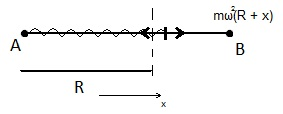
\includegraphics[height=30mm]{3_33.jpg}\\
	$(\omega_1^2 - \omega_0^2)^2 + 4 \beta^2 \omega_1^2 = (\omega_2^2 - \omega_0^2 + 4 \beta^2 \omega_2^2)$\\
	$\omega_1^4 - 2 \omega_0^2 \omega_1^2 + \cancel{\omega_0^4} + 4 \beta^2 \omega_1^2 = \omega_2^4 = 2 \omega_2^2 \omega_0^2 +\cancel{\omega_0^4} + 4 \beta^2 \omega_2^2$\\
	$\omega_0^2 = \frac{\omega_2^4 - \omega_1^4}{2 (\omega_2^2 - \omega_1^2)} + 2 \beta^2 = \frac{\omega_1^2 + \omega_2^2}{2} + 2 \beta^2$\\
	$\omega_{рез}^2 = \omega_0^2 - 2 \beta^2 = \frac{\omega_1^2 + \omega_2^2}{2}$\\
}

